\documentclass[10pt,twocolumn,letterpaper]{article}

\usepackage{cvpr}
\usepackage[utf8]{inputenc}
\usepackage{gensymb}
\usepackage{graphicx}
\usepackage{mathtools}
% TODO: change the image folder
\graphicspath{ {report2-imgs/} }
\usepackage{float}

\cvprfinalcopy
\def\cvprPaperID{a1700831}


% begin of document
\begin{document}
\title{Assignment 2 - Method for Face Detection by Viola and Jones}
\author{Yuanzhong Xia\\
University of Adelaide\\
SA, Australia\\
{\tt\small a1700831@student.adelaide.edu.au}
}
\maketitle

% abstract
\begin{abstract}
This assignment 2 report describes the Viola and Jones's method{\cite{origin}} which can detect a specified object very rapidly.
Their method uses a machine learning method named AdaBoost \cite{adaboost} to both select
% TODO: !!!!!!!!!!!!

\end{abstract}


\section{The Problem}
The problem is to detect face(s) in an input image, and output the image with each face marked with a bounding box.
Although it looks very simple and we don't need to recognize a specific face, the challenge is to detect all the faces in real time.
Because in any normal image, there are so many possible positions and sizes for a single face,
and it's impossible to try every sub-window of them due to the huge computational cost.

Moreover, an input image is not always predictable. The head direction, face integrity, environmental light brightness,
camera features, image quality, etc. can often bring issues to the face detection problem.
And to simplify the problem, the method from Viola and Jones demonstrates with a frontal face detection system,
which means the effects of ``head direction'' and ``face integrity'' are ignored.

\section{Background} \label{sec:bg}
% TODO: describe the competing approaches to the problem


\section{Viola and Jones's Method}
Viola and Jones's method is designed to be applied in any object detection case, and the detection speed is extremely fast around the publish year (2001).
In the paper, all details of the algorithm are demonstrated in doing face detection.
Comparing to other face detection methods whose speeds are faster than Viola and Jones's method,
those methods' speeds are based on checking image difference between the adjacent frames,
while Viola and Jones's method in the demo proceeds each frame independently which means it can achieve even higher speed using the frame difference.

The method has three main steps:
\begin{enumerate}
    \item Compute integral image and Harr-like features;
    \item Construct a classifier by selecting important features using AdaBoost;
    \item Combine classifiers complex classifiers into a cascading structure;
\end{enumerate}

The final cascading classifiers are the final model, classifiers in each layer can reject most features.
Therefore, the computing time gets reduced significantly.

\subsection{Computing features} \label{sec:cf}
The features used in this paper are Haar basis functions motivated by Papageorgiou et al.'s work. (mentioned in Section \ref{sec:bg})
The features are represented in a rectangle split into two, three or four. Then, divide the sub-rectangles into two classes: A and B.
The feature is calculated by the difference of the sum of all pixels marked under class A and the sum of all pixels marked under class B.

To calculate the features, the authors introduce an ``integral image'', which is an array with the same size of the original image ($width \times height$).
Unlike the image pixel array, each cell of the integral image array stores the accumulated pixel sum from top left to current pixel in original image.

Having integral image, the features can be calculated easily in $O(width \times height)$ time,
each sub-rectangle can be easily calculated just by subtracting related integral image cells.
In the paper, the rectangles are tried in each multiply of 24x24 area (i.e. 24x24, 48x48, etc. areas in input images).
Therefore, the exhaustive search set is super large even for a normal images. (For a 384x288 image, the set contains around 180,000 features.)

\subsection{Constructing classifiers}
As is mentioned in Section \ref{sec:cf}, the exhaustive set is super large, and it's impossible to detect every single rectangular feature.
The idea is to select only key features in an image, which can significantly produce the correct prediction result.
And therefore, the time cost will get reduced.

% TODO: The idea is using a simple classifier (in AdaBoost, called weak learner) to select only the key features in an image, which can significantly produce the prediction results.

\subsubsection{Selecting important features}
In selecting important features part, the authors used their previous work \cite{imgret}.
In that method, some features are firstly selected as highly selective features(HSF) which are based on their even previous work \cite{imgdb}.
HSF are a such set of features that they can respond to only a small percentage of images in the input (e.g. 5\%).
The respond in practical means applying convolutions between HSF and input can produce very large numerical values, and it is very efficient.

Additionally, due to the rarity of those features, they use AdaBoost to select and examine HSF.
For each weak learner in that AdaBoost, it computes a two class Gaussian model for the positives and negatives,
and returns the feature for which the model is most sensitive. Figure \ref{img:hsf} shows a set of HSF.

\begin{figure}[t]
    \begin{center}
        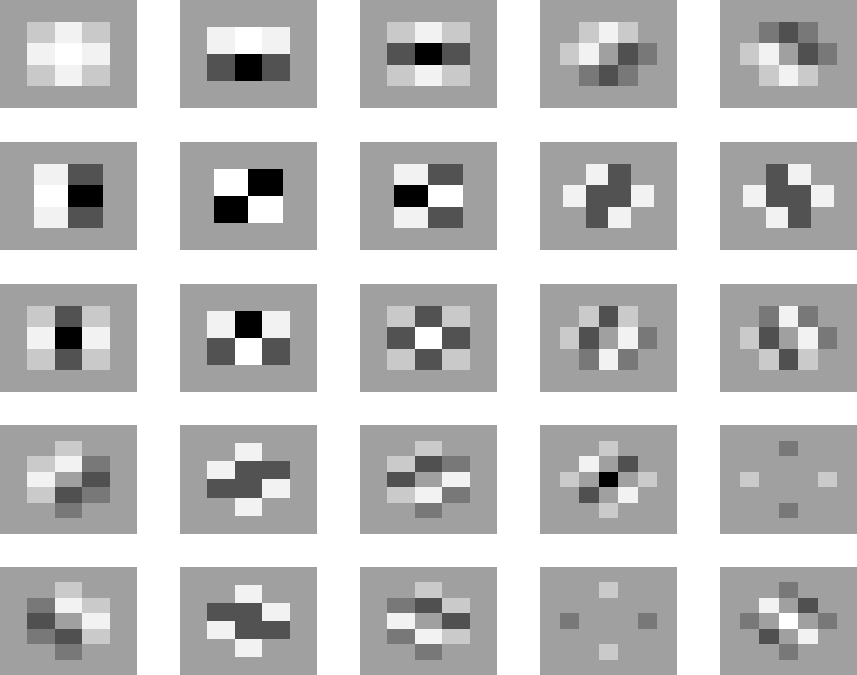
\includegraphics[width=0.9\linewidth]{highly-selective-features}
    \end{center}
    \caption{Sample highly selective features from Viola's previous paper \cite{imgret}}
    \label{fig:hsf}
\end{figure}

\subsubsection{Building classifiers for selected features}

Therefore in practise, the algorithm selects single rectangle features which can best separates the faces and non-faces.
The most important indicator of the resulting classifier is the ``optimal threshold'' which can achieve minimum number of examples are misclassified.
So, in each round of AdaBoost algorithm, only the most optimal threshold is selected for the weak classifier (weak learner).

In the paper, the weak learners are in this form:
\begin{equation}
\label{eq:hjx}
h_{j}(x)=\left\{\begin{matrix*}[l]
1 & \textup{when} \; p_{j}f_{j} < p_{j}\theta _{j}\\
0 & \textup{otherwise}
\end{matrix*}\right.
\end{equation}
where $h_{j}(x)$ is the $j$-th classifier among AdaBoost's final strong classifiers, and $x$ is a 24x24 pixel rectangle of an image.
$p_{j}$ is used to mark the positive (1, representing face) and negative (-1, representing non-face).
$f_{j}$ is a Haar-like features, and a threshold $\theta _{j}$ is used for best separating positive and negative features.

In the demonstration from the paper, the all the 24x24 pixel rectangles are marked positive in an with-face image,
whereas all the 24x24 pixel rectangles are marked negative in a non-face image.
The error rates of the weak learners selected in early round can often achieve between 0.1 to 0.3 which is quite good.
However, when entering later rounds, the error rates increase to around 0.5.

Combining all the weak learners, the final classifier will be:
$$h(x)=\left\{\begin{matrix*}[l]
1 & \textup{when} \; \sum_{t=1}^{T} \alpha _{t} h_{t}(x) \geq \frac{1}{2} \sum_{t=1}^{T} \alpha _{t}\\
0 & \textup{otherwise}
\end{matrix*}\right.$$
where $\alpha _{t}$ is calculated by accumulated weighted error rate which is calculated during the procedure of selecting weak learners in AdaBoost algorithm.
$h_{i}(x)$ is the weak learner mentioned in Equation (\ref{eq:hjx}). $T$ is the total round number, which is also the number of weak learners.
In the paper, the number of $T$ depends on the current layer (which will be discussed in Section \ref{sec:bcc}).

\subsection{Building cascading classifiers} \label{sec:bcc}

% TODO: the total round of AdaBoost

\section{Hypothesis}
% \subsection{Limitation and Improvements}
% https://blog.bluecrossmn.com/future-face-minnesota-look-willmar/ - the picture source
% http://web01a.elitedaily.com/envision/photographer-brilliantly-captures-the-many-different-facial-expressions-we-all-go-through-photos/

AdaBoost can always overfit if the fit process keeps going on

In second step: no single feature can work perfectly, but the combination of selected features can works perfectly

Although, the features selected (xxx) shown in the Figure 4 are xxxx, they are still automatically selected by AdaBoost!
therefore, the performance is fully depending on the training data.

The prediction result is very stable, using the same model to predict will always get the same result.

% TODO: how to come over the slightly tilted face (the Haar basis features can do that)
In principle, any kind of face can be detected if the training data have this

% TODO: the OpenCV implementation, the different models
% TODO: the training data is unknown although I searched for XXXXXX

\section{Experiments}

\section{Extensions}
% TODO: the adjacent frames difference used in video face detection
% only recalculate the different parts

%

\section{Conclusion}

% Bibliography
\begin{thebibliography}{9}
\bibitem {origin}
P. Viola and M. Jones, ``Rapid object detection using a boosted cascade of simple features,''
In \textit{Proc. IEEE Conf. Comput. Vis. Pattern Recog.}, 2001, pp. 511–518.

\bibitem {adaboost}
Y. Freund and R.E. Schapire, ``A decision-theoretic generalization of on-=line learning and an application to boosting,''
In \textit{Computational Learning Theory: Eurocolt '95}, pages 23-27, Springer-Verlag, 1995.

\bibitem {imgret}
K. Tieu and P. Viola, ``Boosting image retrieval,''
In \textit{Proceedings of the IEEE Conference on Computer Vision and Pattern Recognition}, 2000.

\bibitem {imgdb}
J. S. DeBonet and P. Viola, ``Structure driven image database retrieval,''
In \textit{Adv. Neur. Info. Proc. Sys.}, volume 10, 1998.


\end{thebibliography}

\end{document}
